\documentclass{beamer}
\usepackage[italian]{babel}
\usetheme{Berkeley}
\usepackage{graphicx}
\usepackage{booktabs}
\graphicspath{{figures/}}

\title{Condividere informazioni in modo \\
sicuro combinando Git e Blockchain}
\author{Studente: Paolo Speziali \\ Relatore: Luca Grilli}
\institute{Università degli Studi di Perugia - Dipartimento di Ingegneria\\Corso di laurea triennale in Ingegneria Informatica ed Elettronica\\[\medskipamount]
      
\includegraphics[width=0.3\textwidth]{figures/logo_unipg.png}
 }
\logo{
\includegraphics[height=1cm]{favicon.png}}
\date{A.A. 2020/2021}

\begin{document}
\begin{frame}
	\titlepage % beamer's \maketitle
\end{frame}
\begin{frame}
	\frametitle{Indice}
	\tableofcontents
\end{frame}
\section{Il Problema}
\begin{frame}
	\frametitle{La digitalizzazione}
	È in atto, negli ultimi anni, un piano di \textbf{digitalizzazione} delle PA.
	Esso mira all'evoluzione tecnologica di tutte le sue mansioni e alla creazione
	di portali web per il cittadino.
	L'esigenza di questa trasformazione si è fatta sentire anche da parte
	dell'\textbf{Unione Europea}, che con il \textbf{Recovery Fund}
	ci sta fornendo i fondi per attuarla, ben \textbf{11,75 milioni di euro}.
	\begin{figure}
		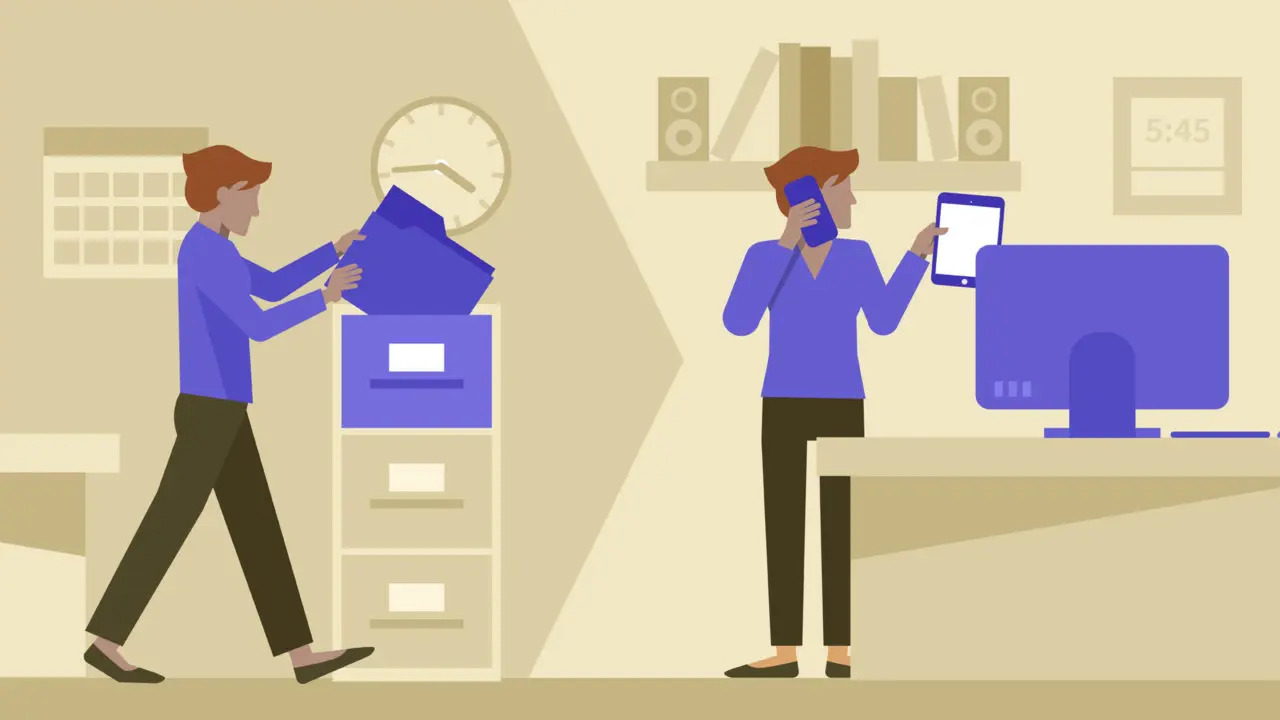
\includegraphics[width=0.55\textwidth]{digitalizzazione.jpg}
		% https://www.agendadigitale.eu/documenti/digitalizzazione-della-pa-in-italia-la-strategia-delle-tre-c/
	\end{figure}
\end{frame}

\begin{frame}
	\frametitle{Il problema della burocrazia}
	Il più grande avversario della digitalizzazione è la \textbf{burocrazia} italiana:
	i suoi processi sono \textbf{lenti} e \textbf{complessi} anche a causa dell'\textbf{importanza}
	dei documenti da gestire.
	È necessaria una \textbf{sburocratizzazione}
	grazie a degli strumenti digitali che permettano di \textbf{salvare},
	\textbf{validare} e \textbf{condividere} documenti senza abbassare il \textbf{livello di sicurezza}.
	\medskip
	\begin{figure}
		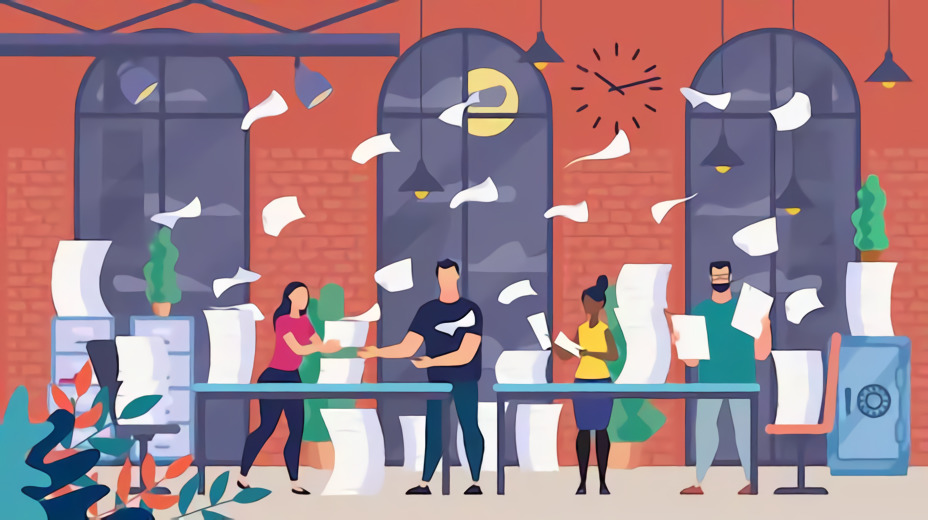
\includegraphics[width=0.65\textwidth]{buro.jpg}
		% https://www.identitafutura.it/burocrazia-allitaliana/
	\end{figure}
\end{frame}

\begin{frame}
	\frametitle{Gli strumenti attuali}
	\medskip
	\begin{columns}
		\column{0.65\textwidth}
		Uno strumento digitale solitamente segue uno di questi due paradigmi:
		\textbf{centralizzato} e \textbf{distribuito}. \\
		Nel primo un'entità centrale si occupa dell'\textbf{immagazzinamento} e della \textbf{verifica} dei dati
		degli utenti.\\ Ciò ha diversi \textbf{svantaggi}:
		\begin{itemize}
			\item Potenziali attacchi all'entità
			\item Possibile uso malevolo dei nostri dati
			\item Alti costi d'intermediazione
		\end{itemize}
		\column{0.35\textwidth}
		\begin{figure}
			
\includegraphics[width=0.90\textwidth]{cent.png}
			% https://icon-icons.com/it/icona/centralizzato-rete-dati-blockchain-tecnologia/95906
		\end{figure}
	\end{columns}
\end{frame}

\begin{frame}
	\frametitle{Strumenti distribuiti}
		Usando invece \textbf{un'architettura distribuita}, sia per la gestione dei file,
		sia per la verifica delle informazioni, saremo in grado costruire uno strumento
		che può affidarsi alla parola di una moltitudine di entità, rendendo molto
		più complicati e rilevabili attacchi e manomissioni.
	\medskip
	\begin{figure}
		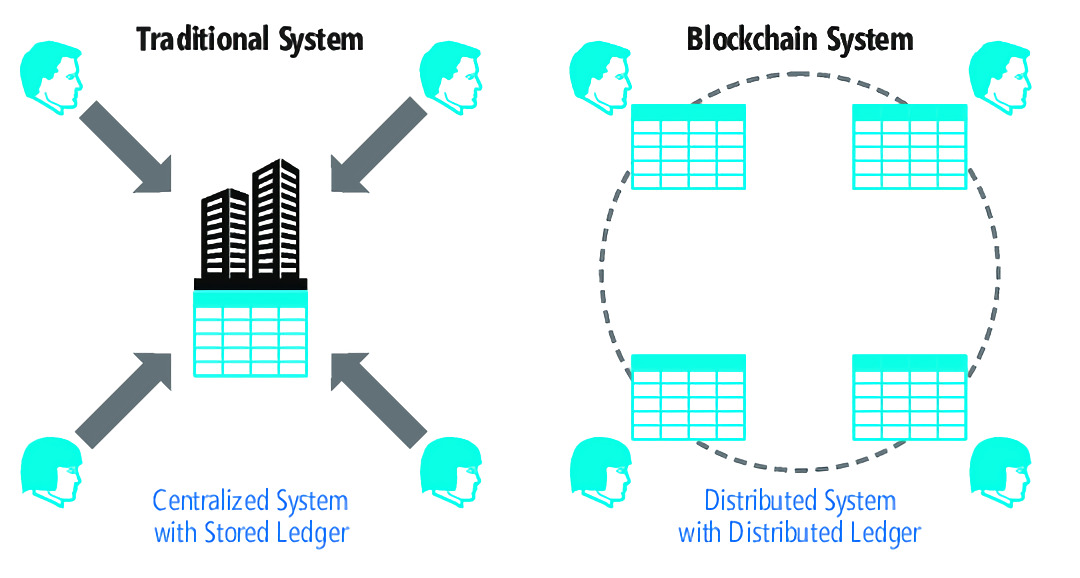
\includegraphics[width=0.70\textwidth]{dece.jpg}
		% https://docs.microsoft.com/it-it/archive/msdn-magazine/2018/july/blockchain-decentralized-applications-with-azure-blockchain-as-a-service
	\end{figure}
\end{frame}

\section{Concetti preliminari}
\begin{frame}
	\frametitle{Funzioni crittografiche di hashing}
	Una funzione crittografica di hashing è una funzione di hashing, ovvero
	una funzione che permette di associare,
	a una qualsiasi sequenza \(m\) di lunghezza arbitraria in input, una sequenza
	in output \(h(m)\) di lunghezza costante,
	con alcune proprietà aggiunte che deve seguire per poter essere considerata
	\emph{crittograficamente sicura}. Esse impediscono di risalire all'input originale
	e facilitano i \textbf{controlli di integrità sui file}.
	\begin{figure}
		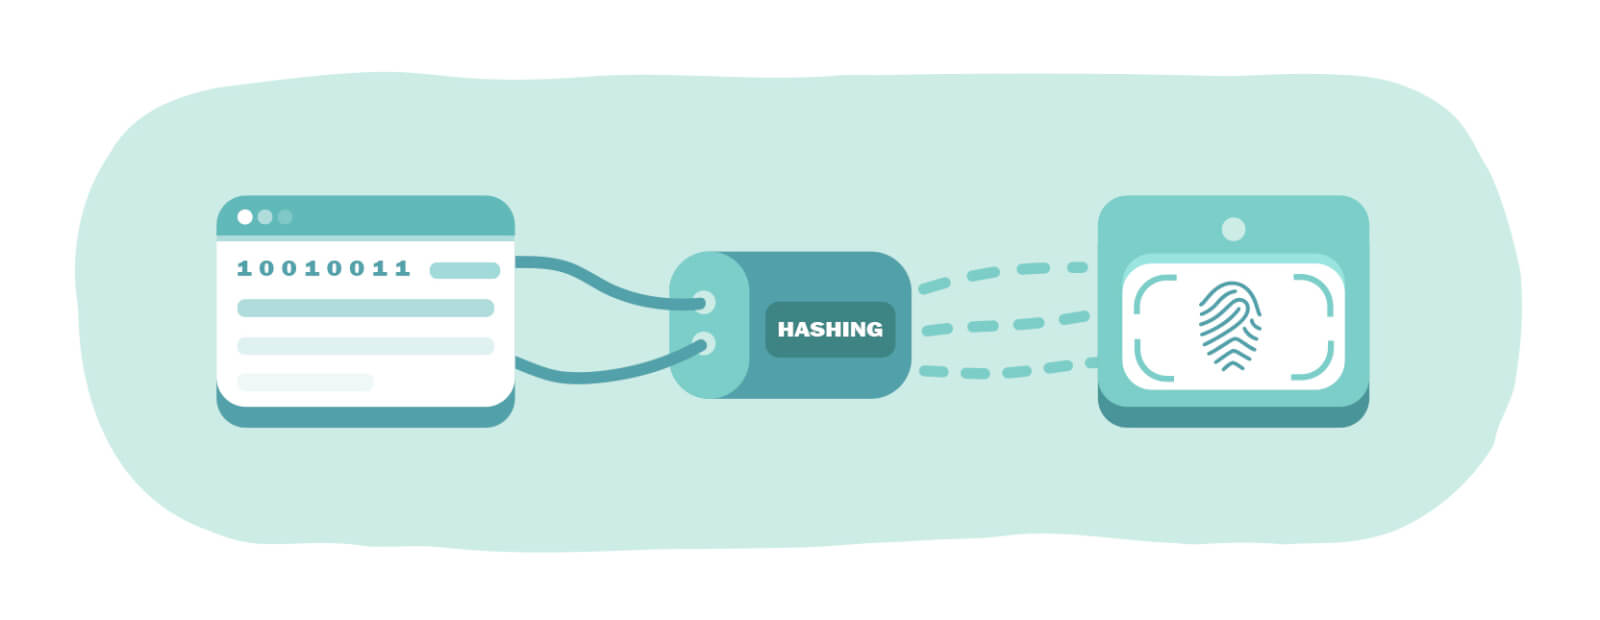
\includegraphics[width=0.85\textwidth]{figures/hashing.jpg}
	\end{figure}
\end{frame}

\begin{frame}
	\frametitle{Git}

	\begin{columns}[T]
		\column{0.99\textwidth}
		\textbf{Git} è  è il sistema di controllo di versione (\textbf{VCS}) \\
		distribuito più diffuso al mondo. \\
		Un VCS suddivide gli insiemi di file e directory\\ in repository.
		Git modella ogni repository\\come una \emph{sequenza di snapshot} 
		di un piccolo\\ file system.
		Ogni volta che un utente salva lo stato del suo progetto
		(tramite l'operazione di \emph{commit}), Git crea uno snapshot
		di tutti i file e le directory sotto controllo di versione in
		quel momento e lo archivia nel suo database locale.
		Inoltre, quasi ogni operazione di Git va ad aggiungere informazioni
		al suo database, anche se si tratta
		di un'operazione di rimozione, ciò assicura che ogni cambiamento
		sia reversibile.
		\column{0.01\textwidth}
		\hspace*{-2cm}
		
\includegraphics[width=2cm]{figures/git.png}
	\end{columns}

\end{frame}

\begin{frame}
	\frametitle{Blockchain}
	La \textbf{blockchain}\dots
	\medskip
	\begin{figure}
		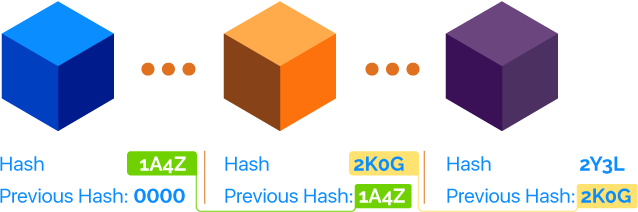
\includegraphics[width=0.65\textwidth]{figures/blockchain.png}
		% https://www.esperiabc.com/it/blockchain-e-sicurezza-informatica/
	\end{figure}
\end{frame}

\begin{frame}
	\frametitle{Accumulatori crittografici}
	\begin{columns}
		\column{0.62\textwidth}
		Gli \textbf{accumulatori crittografici} sono strumenti che permettono
		di comprimere molti elementi informativi in una costante di dimensione fissa.
		
		Un esempio ne sono i \textbf{Merkle Tree}, alberi binari
		in cui ogni foglia corrisponde all'hash di un elemento.
		Risalendo verso la radice ogni nodo interno calcolerà il proprio hash
		concatenando gli hash dei nodi figli, infine si otterrà
		una radice (\textbf{Merkle Root} o MR), univoca
		a quella lista di elementi che l'albero
		ha come foglie, in quella sequenza.
		\column{0.38\textwidth}
		\begin{figure}
			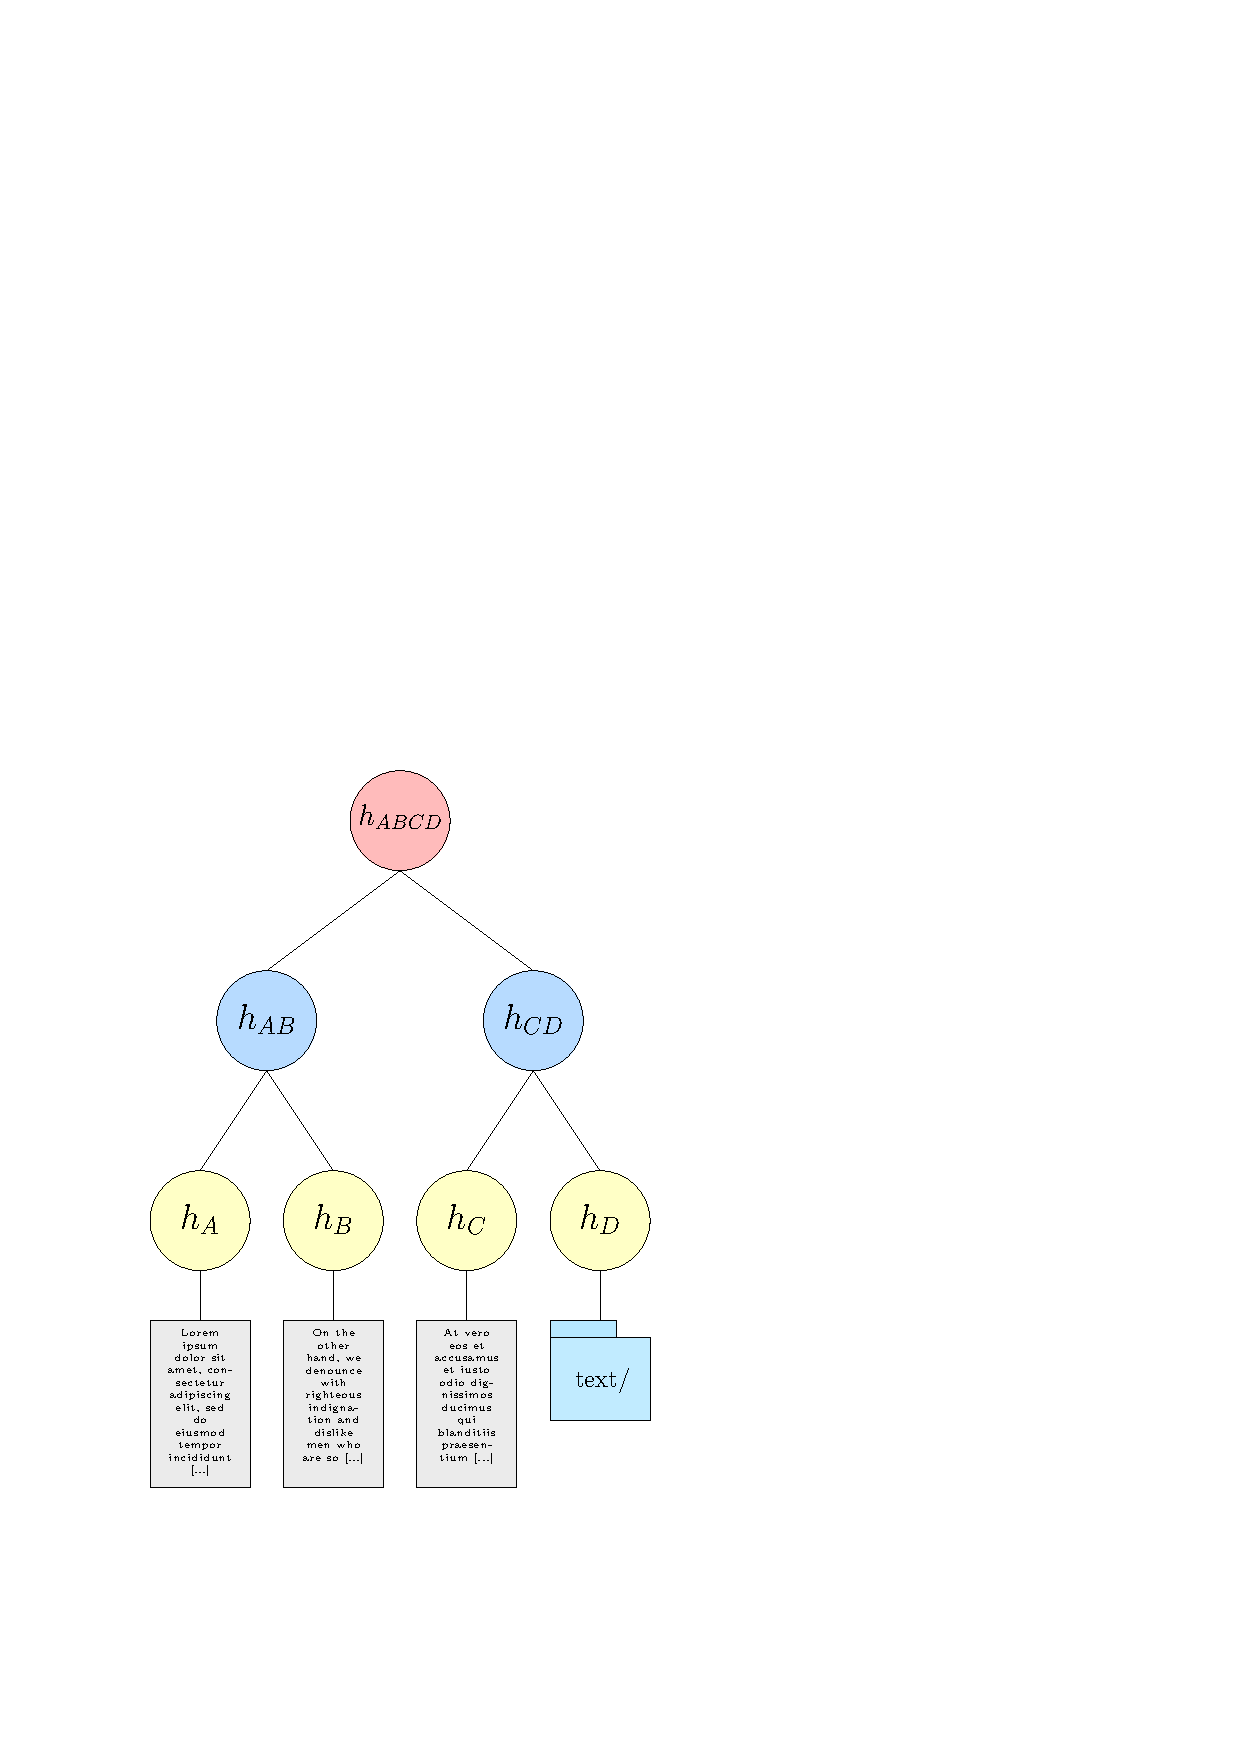
\includegraphics[width=0.9\textwidth]{figures/mt1.pdf}
		\end{figure}
	\end{columns}
\end{frame}

\section{L'Obiettivo}
\begin{frame}
	\frametitle{L'Obiettivo}
	Il sistema progettato ha lo scopo di riuscire a fornire a chi ne usufruisce
	un livello di sicurezza aggiuntivo sopra il software Git tramite un'opportuna
	comunicazione con la blockchain.

	Il software, grazie a un'interfaccia user-friendly, deve permettere non solo di gestire
	le directory come normali repository, ma fornire
	anche degli utili strumenti di salvataggio di hash su blockchain,
	esportazione di sottoinsiemi di repository
	e verifica sia di singoli file che di moltitudini.
	Tutto ciò implementato con operazioni più o meno severe (e quindi onerose)
	e con un occhio di riguardo anche alla quantità di
	dati da memorizzare durante l'implementazione.
\end{frame}

\begin{frame}
	\frametitle{Perché blockchain?}
	L'utilizzo della blockchain nel progetto è giustificato da:
	\begin{itemize}[<+->]
		\item Natura condivisa \(\rightarrow\) Transazioni facilmente tracciabili
		\item Decentralizzazione \(\rightarrow\) Resistenza allo \textbf{SPOF}\footnote{Single Point Of Failure}
		\item Immutabilità \(\rightarrow\) Garantisce integrità dei dati
		\item Validazione \emph{peer-to-peer} \(\rightarrow\) Potere distribuito
		\item Disintermediazione \(\rightarrow\) Eliminazione di \emph{middle-men} e dei loro costi
	\end{itemize}
\end{frame}

\begin{frame}
	\frametitle{Il costo della blockchain}
	Il salvataggio delle informazioni su blockchain ha però un costo proporzionale al quantitativo
	di dati che vorremo memorizzarci.
	
	Per superare questo problema dovrà essere implementata una soluzione che sfrutti
	degli accumulatori crittografici per memorizzare l'identità di molti collettivi di documenti
	con un unico hash.

	Ovviamente la loro struttura dovrà essere tale da permetterci di andare a reperire
	informazioni passate e già calcolate in un tempo che sia relativamente ragionevole.
\end{frame}

\section{Il Software PineSU}
\begin{frame}
	\frametitle{Il Software PineSU}
	\begin{columns}
		\column{0.7\textwidth}
		Un'implementazione del sistema ideato è l'applicativo \textbf{PineSU}. \\
		PineSU è un software \emph{lightweight} in Javascript e che sfrutta il runtime Node.js.
		L'applicazione va a considerare gli insiemi di file come delle entità chiamate
		\textbf{Storage Unit} (SU) con cui va ad inglobare logicamente una repository Git,
		costruendo, tramite metadati, una struttura introno ad essa.
		Queste SU sono le unità su cui si andranno ad effettuare le singole
		operazioni, eccetto la registrazione su blockchain che si svolgerà
		collettivamente con l'ausilio di accumulatori crittografici. 
		\column{0.3\textwidth}
		\centering
		\begin{figure}
			
\includegraphics[width=\textwidth]{figures/favicon.png}
		\end{figure} 
	\end{columns}
\end{frame}

\begin{frame}
	\frametitle{Workflow}
	\centering
	\begin{figure}
		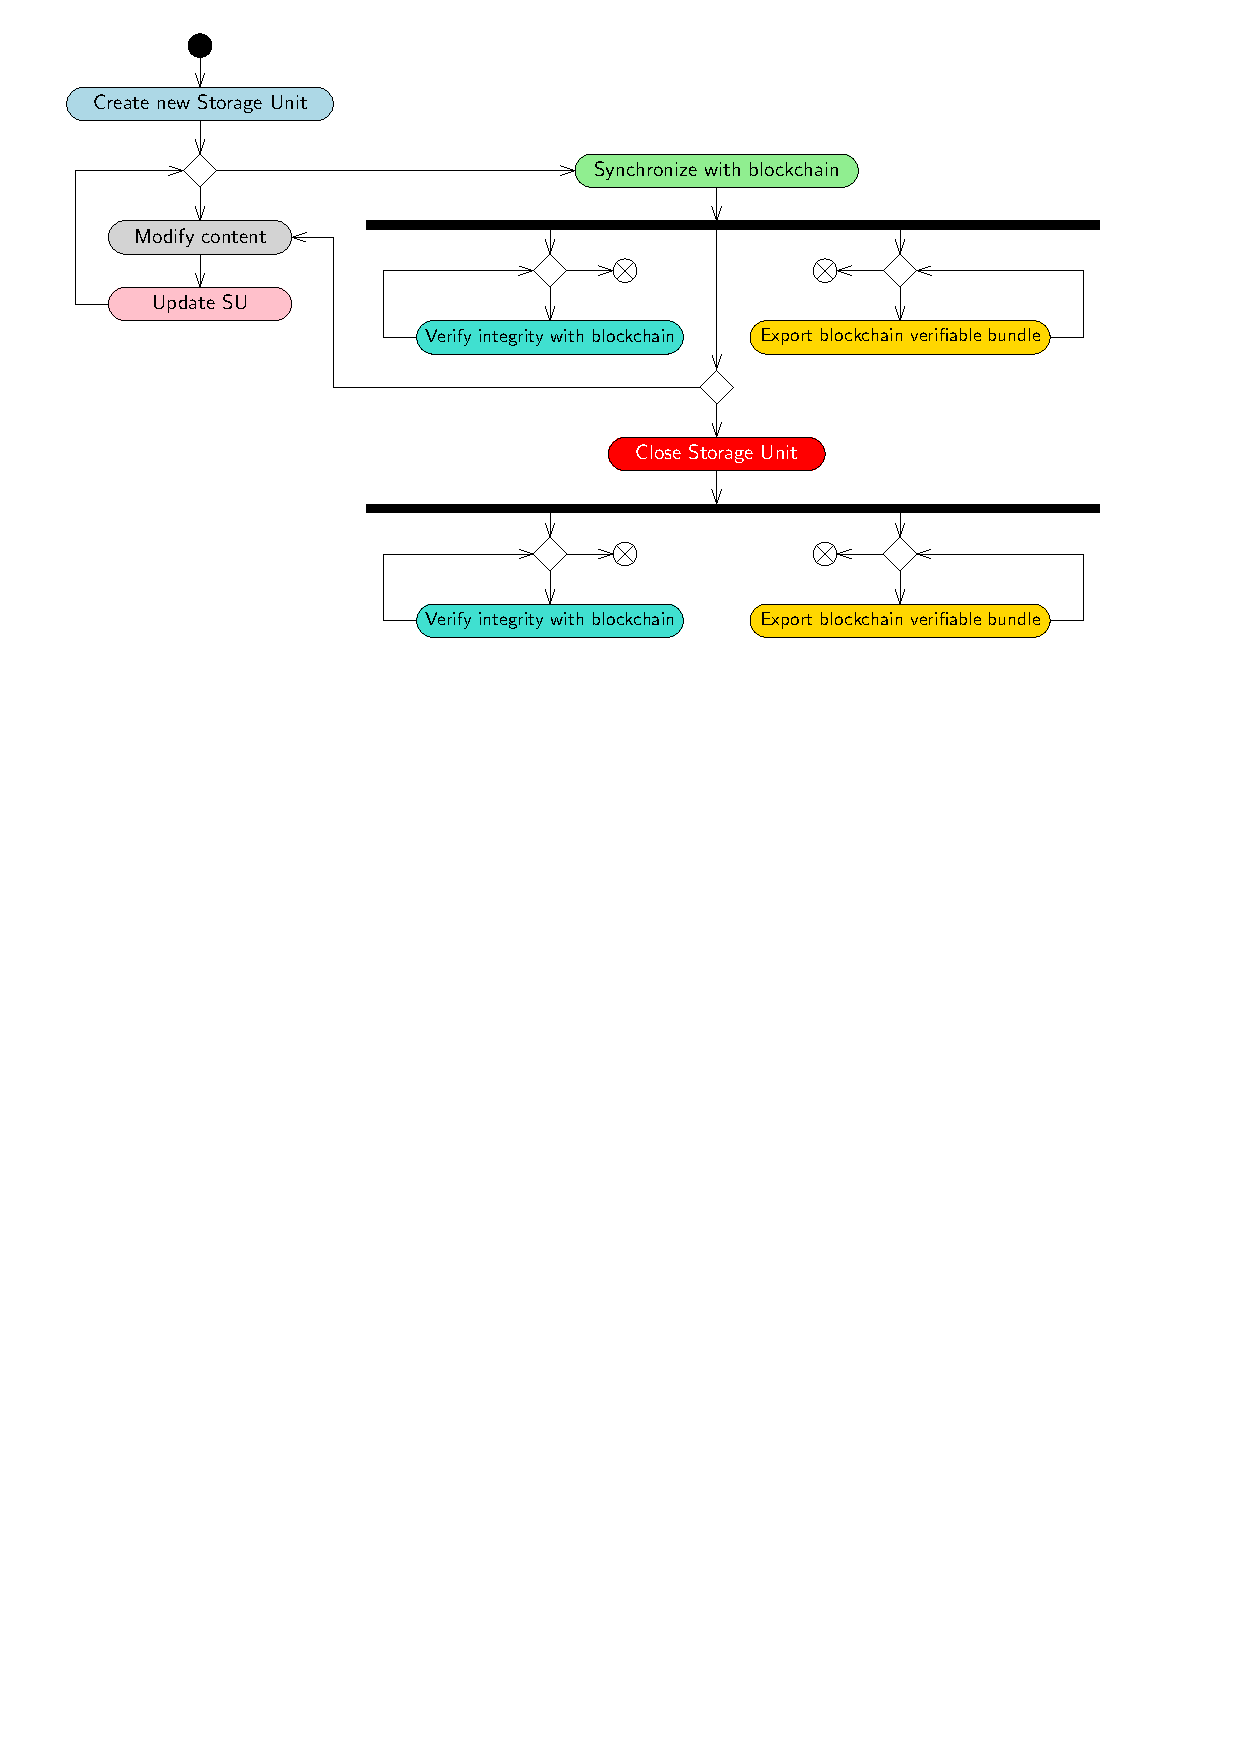
\includegraphics[width=\textwidth]{figures/activityDiag.pdf}
	\end{figure}
\end{frame}

\begin{frame}
	\frametitle{Ciclo vitale di una Storage Unit}
	\centering
	\begin{figure}
		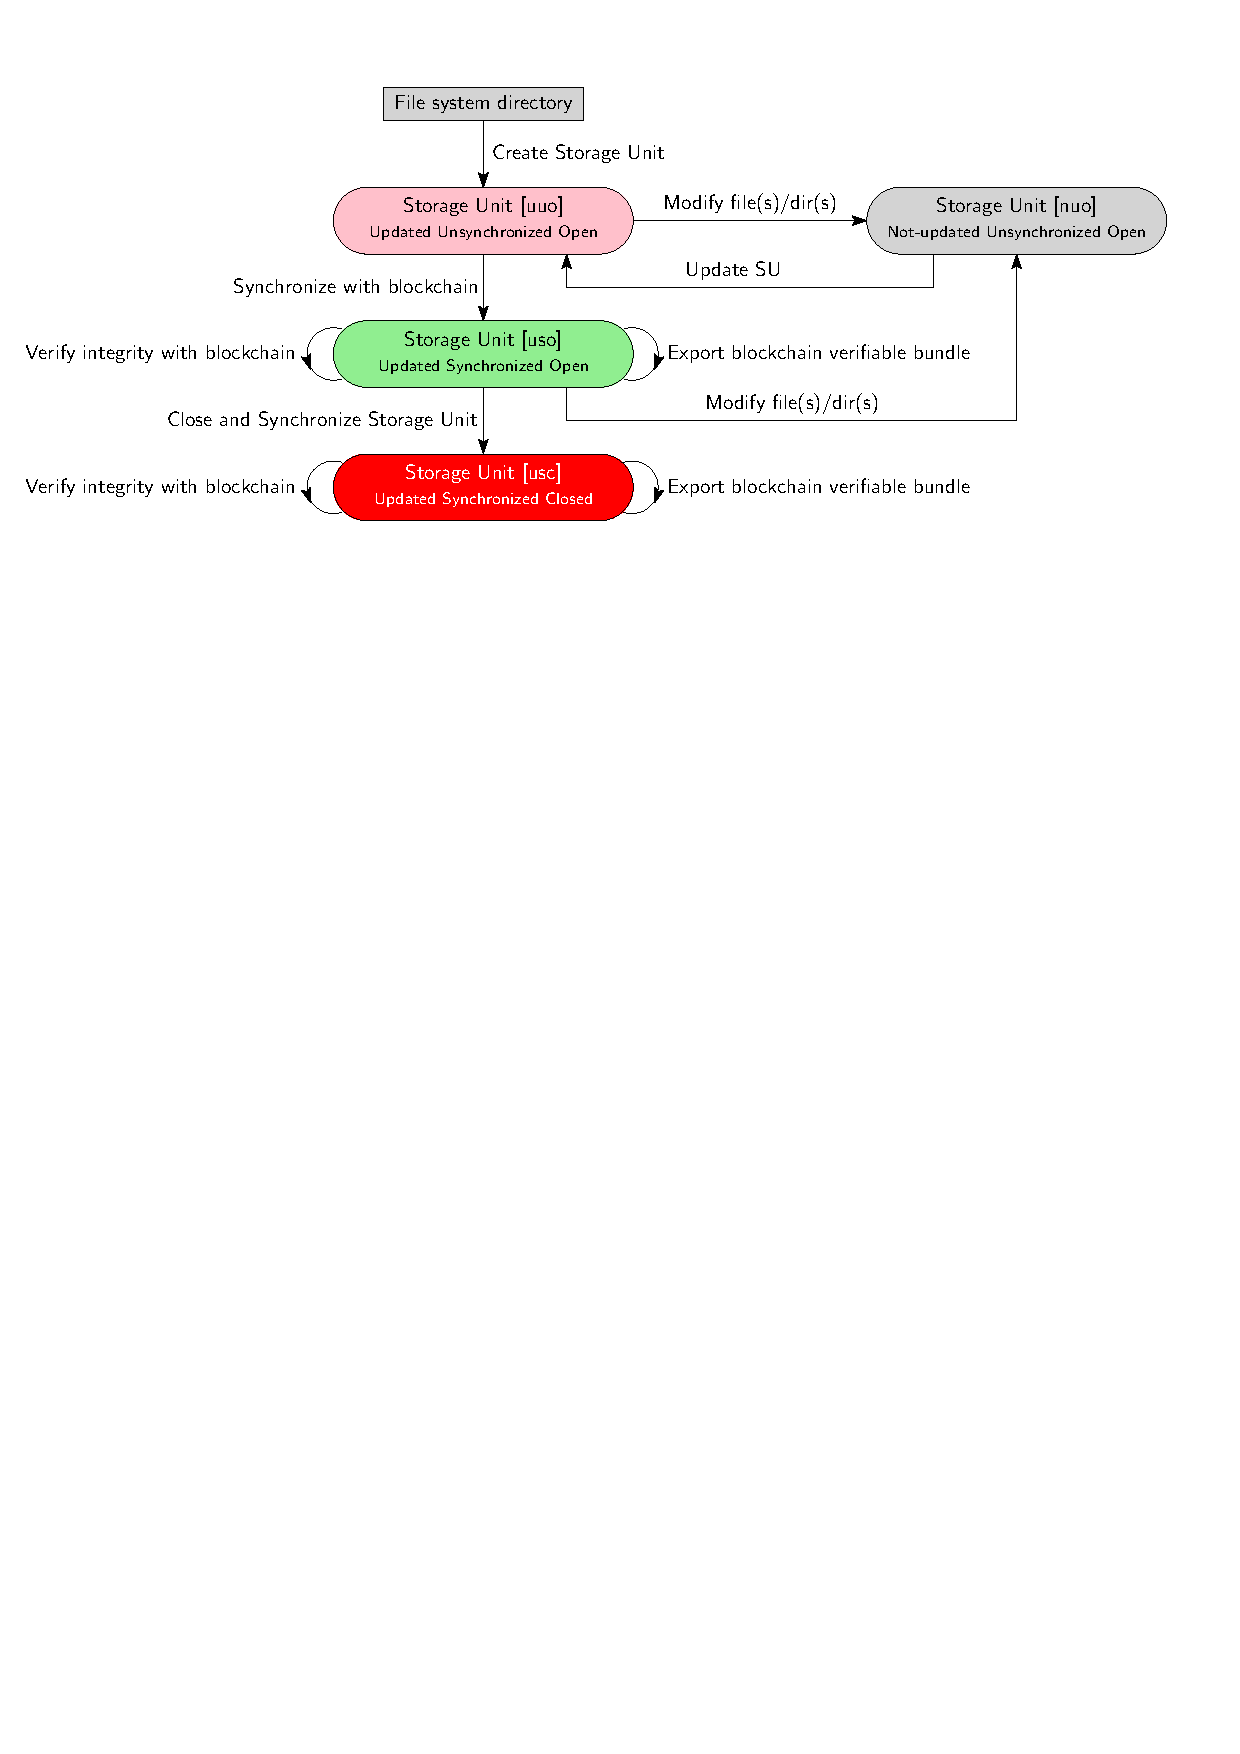
\includegraphics[width=\textwidth]{figures/stateDiag2.pdf}
	\end{figure}
\end{frame}

\begin{frame}
	\frametitle{Architettura}
	\centering
	\begin{figure}
		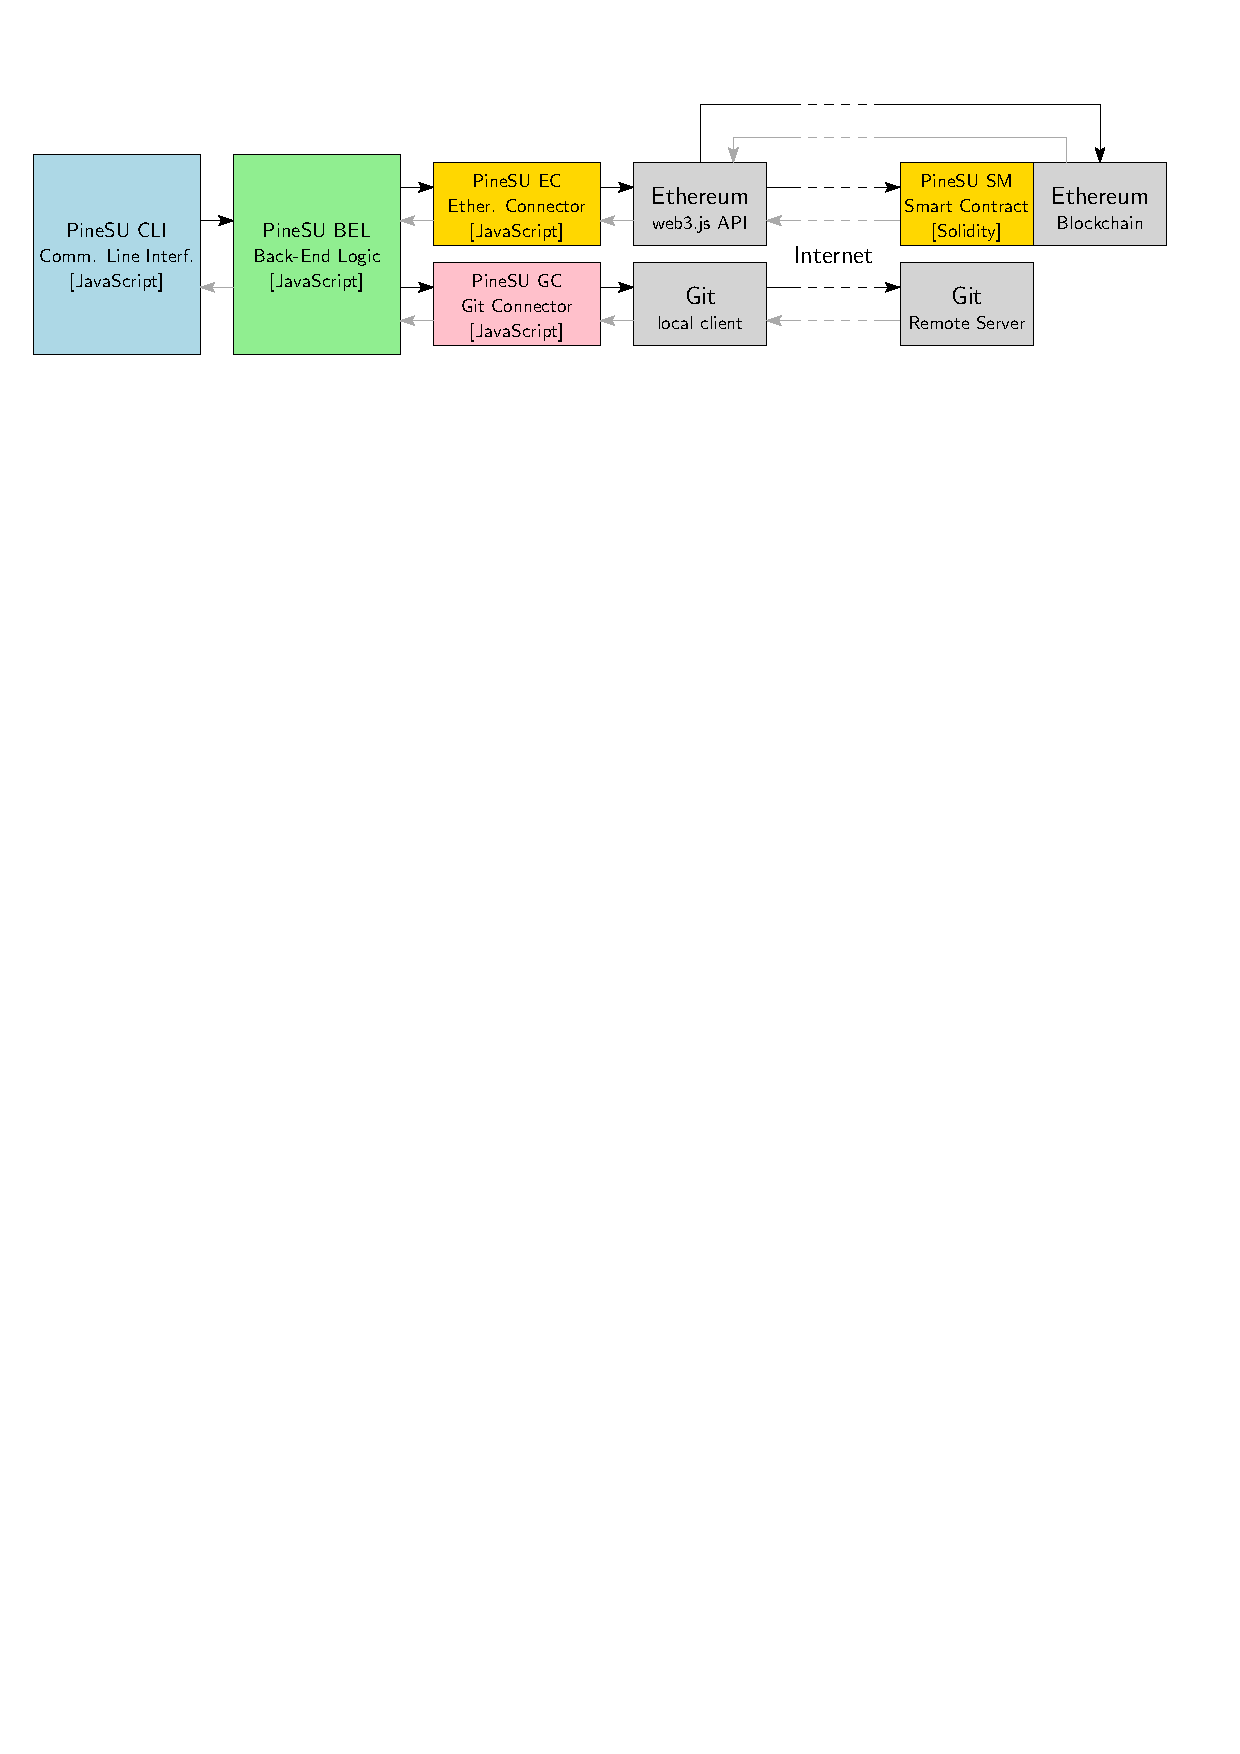
\includegraphics[width=\textwidth]{figures/pineSU-architecture.pdf}
	\end{figure}
\end{frame}

\begin{frame}
	\frametitle{Architettura (Cont.)}
	\begin{itemize}
		\item \emph{PineSU \textbf{CLI} (Command Line Interface)}: Modulo che crea l'interfaccia utente con cui è possibile
			interagire e richiama le funzioni degli altri moduli di conseguenza.
		\item \emph{PineSU \textbf{BEL} (Back End Logic)}: Questo componente è il nucleo di PineSU.
		Gestisce tutte le SU e controlla la comunicazione con la blockchain e il client Git locale.
		\item \emph{PineSU \textbf{EC} (Ethereum Connector)}: Si interfaccia con le API della blockchain. 
		\item \emph{PineSU \textbf{GC} (Git Connector)}: Si interfaccia con il client Git. 
		\item \emph{PineSU \textbf{SM} (Smart Contract)}: Permette registrazioni permanenti di singole SU nella blockchain.
	\end{itemize}
\end{frame}

\begin{frame}
	\frametitle{Gli accumulatori di PineSU}
	\begin{columns}
		\column{0.5\textwidth}
		\begin{itemize}[<+->]
			\item \emph{SU Merkle Tree}: Le sue foglie sono gli hash dei file e directory della SU, la sua root è l'hash della SU stessa. 
			\item \emph{Storage Group (\textbf{SG})}: Le sue foglie sono le SU da registrare su blockchain nella prossima transazione. 
			\item \emph{Merkle Calendar (\textbf{MC})}.
		\end{itemize}
		\column{0.5\textwidth}
		\centering
		\begin{figure}
			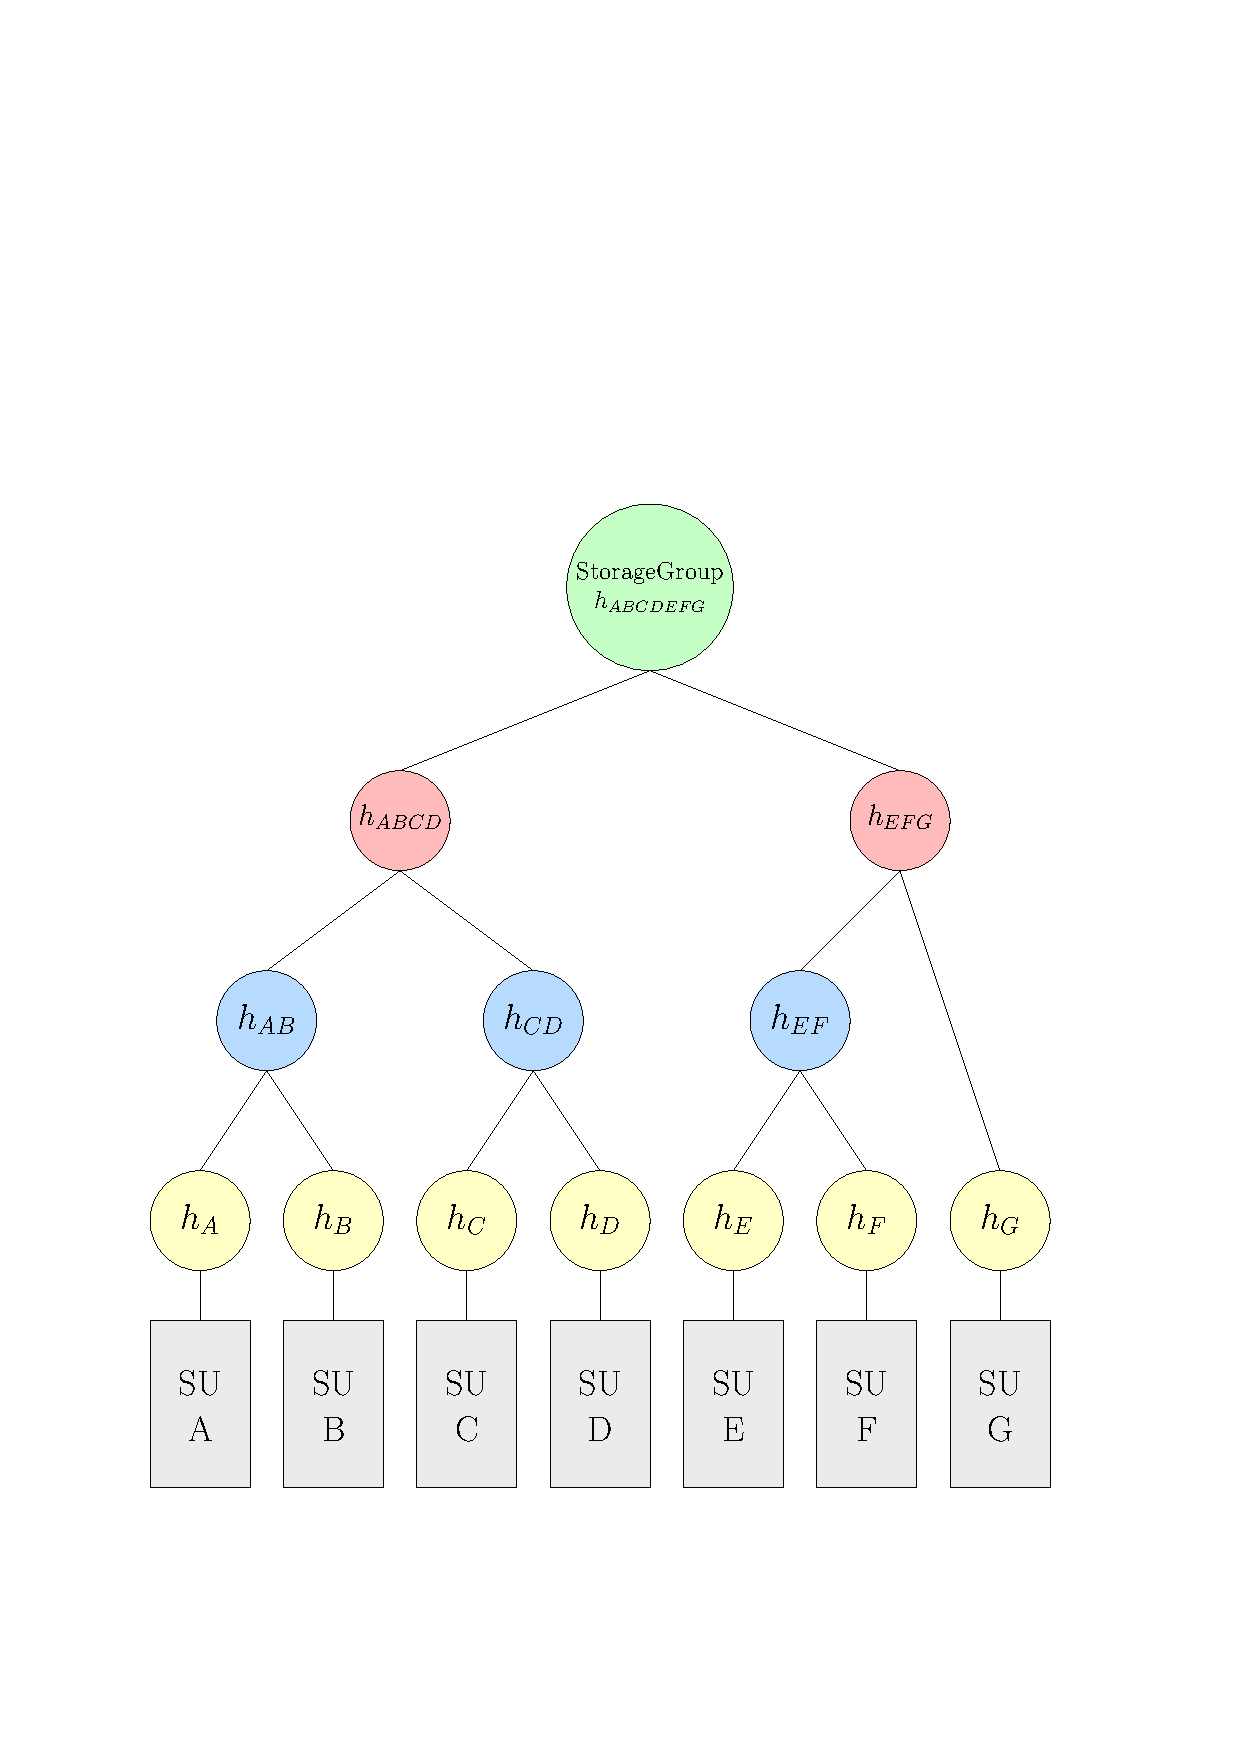
\includegraphics[width=\textwidth]{figures/sg1.pdf}
			\caption{Uno Storage Group}
		\end{figure} 
	\end{columns}
\end{frame}

\begin{frame}
	\frametitle{Gli accumulatori di PineSU (Cont.)}
	\begin{columns}
		\column{0.5\textwidth}
		Un \textbf{Merkle Calendar} è un albero in cui le foglie sono
		i Blockchain Synchronization Point (\textbf{BSP}), istanze di
		Storage Group, a loro volta raggruppate in nodi rappresentanti
		mesi e anni, ciò rende i reperimenti di registrazioni passate
		più agevoli e veloci.
		\column{0.5\textwidth}
		\centering
		\begin{figure}
			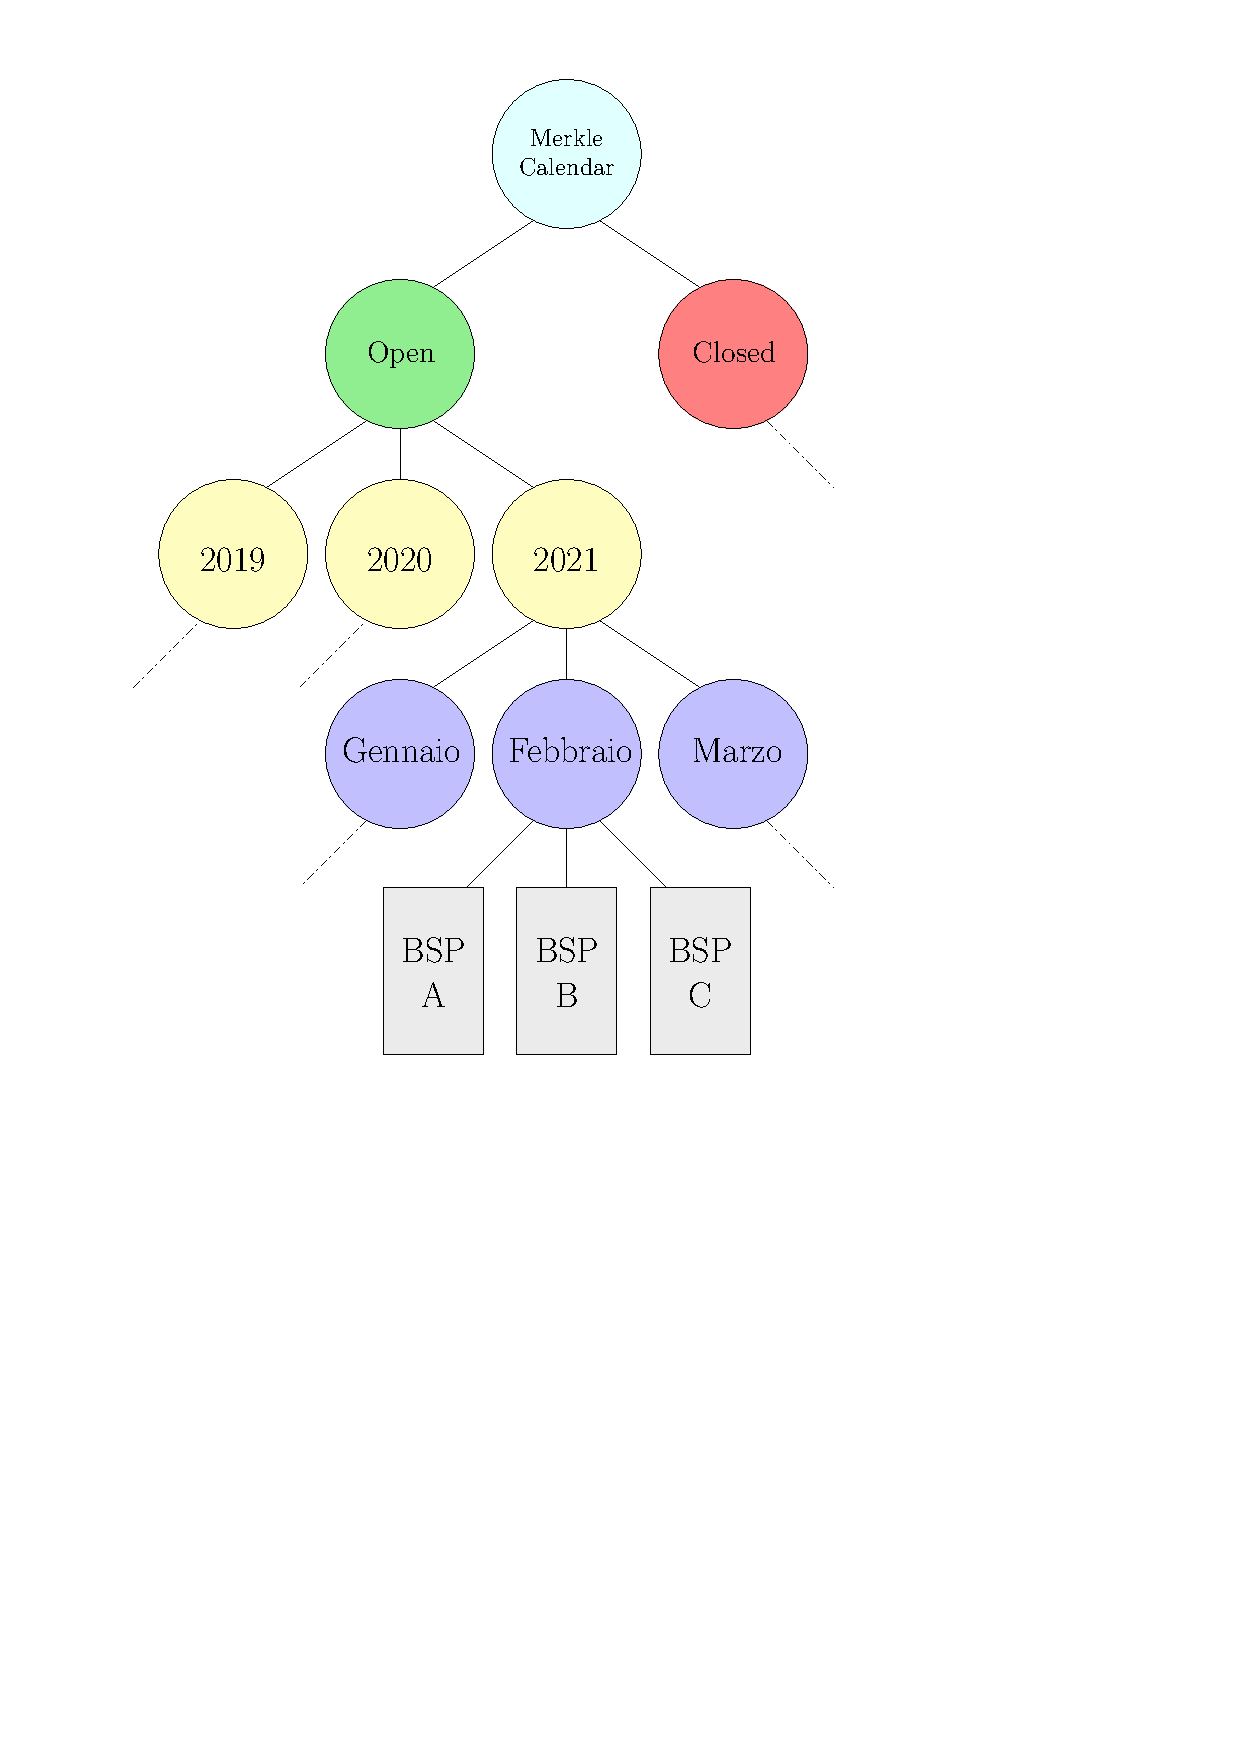
\includegraphics[width=0.8\textwidth]{figures/mc1.pdf}
			\caption{Un Merkle Calendar}
		\end{figure} 
	\end{columns}
\end{frame}

\begin{frame}
	\frametitle{Le operazioni disponibili}
	\begin{enumerate}[<+->]
		\item Creazione di una Storage Unit o Ricalcolo di una Storage Unit pre-esistente
		\item Staging di una Storage Unit nello Storage Group
		\item Registrazione dello Storage Group nella Blockchain
		\item Chiusura di una Storage Unit
		\item Esportazione di sottoinsiemi di file da una SU
		\item Controllo di integrità di singoli file esportati da altre SU
		\item Controllo di integrità su una SU
	\end{enumerate}
\end{frame}

%\section{Fonti}
%\begin{frame}
%	\frametitle{Fonti}
%	\begin{itemize}
%		\item \href{https://ethereum.org/it/developers/}{Strumenti Ethereum per sviluppatori} 
%  		\item \href{https://www.trufflesuite.com/tutorial}{Tutorial Truffle DAPPs - Pet Shop}
%  		\item \href{https://www.sitepoint.com/javascript-command-line-interface-cli-node-js/}{Build a JavaScript CLI with Node.js}
%  		\item \href{https://developer.mozilla.org/en-US/docs/Learn/JavaScript/Asynchronous/Async_await}{Tutorial di Mozilla su async / await}
%  		\item Immagini reperite dai siti ufficiali degli strumenti eccetto per alcune scaricate da queste pagine web:
%			\begin{itemize}
%				\item \href{https://www.poeticoding.com/hashing-a-file-in-elixir/}{Funzioni di Hashing}
%				\item \href{https://www.romatoday.it/attualita/concorso-rai-fiera-roma-norme-covid-19.html}{Concorso pubblico}
%				\item \href{https://www.criptovalute24.com/ethereum-migliora-la-sua-blockchain-rialzo-del-5-4/}{Ethereum Blockchain}
%				\item \href{https://blog.netsons.com/git-software-guida-facile/}{Git repository}
%				\item \href{https://amerlin.keantex.com/programmazione-asincrona-con-async-await-parte-2/}{async / await}
%				\item \href{https://transparency.dev/verifiable-data-structures/}{Merkle Tree}
%			\end{itemize}
%			\item \href{https://waifu2x.booru.pics/Home/index}{Strumento di upscaling delle immagini} 
%	\end{itemize}
%\end{frame}

\end{document}